 \documentclass[bachelor, och, labwork]{shiza}
% параметр - тип обучения - одно из значений:
%    spec     - специальность
%    bachelor - бакалавриат (по умолчанию)
%    master   - магистратура
% параметр - форма обучения - одно из значений:
%    och   - очное (по умолчанию)
%    zaoch - заочное
% параметр - тип работы - одно из значений:
%    referat    - реферат
%    coursework - курсовая работа (по умолчанию)
%    diploma    - дипломная работа
%    pract      - отчет по практике
% параметр - включение шрифта
%    times    - включение шрифта Times New Roman (если установлен)
%               по умолчанию выключен
\usepackage{subfigure}
\usepackage{tikz,pgfplots}
\pgfplotsset{compat=1.5}
\usepackage{float}
\usepackage{pdfpages}

\usepackage{titlesec}
\setcounter{secnumdepth}{4}
\titleformat{\paragraph}
{\normalfont\normalsize}{\theparagraph}{1em}{}
\titlespacing*{\paragraph}
{35.5pt}{3.25ex plus 1ex minus .2ex}{1.5ex plus .2ex}

\titleformat{\paragraph}[block]
{\hspace{1.25cm}\normalfont}
{\theparagraph}{1ex}{}
\titlespacing{\paragraph}
{0cm}{2ex plus 1ex minus .2ex}{.4ex plus.2ex}

% --------------------------------------------------------------------------%


\usepackage[T2A]{fontenc}
\usepackage[utf8]{inputenc}
\usepackage{graphicx}
\graphicspath{ {./images/} }
\usepackage{tempora}
\usepackage{kantlipsum}
\usepackage[sort,compress]{cite}
\usepackage{amsmath}
\usepackage{amssymb}
\usepackage{amsthm}
\usepackage{calrsfs}
\newcommand{\La}{\mathcal{L}}
\newcommand{\Ra}{\mathcal{R}}
\newcommand{\Da}{\mathcal{D}}
\newcommand{\Ha}{\mathcal{H}}
\newcommand{\Ja}{\mathcal{J}}
\usepackage{fancyvrb}
\usepackage{listings}
\usepackage{listingsutf8}
\usepackage{longtable}
\usepackage{array}
\usepackage[english,russian]{babel}

%\usepackage[colorlinks=true]{hyperref}
\usepackage{url}

\usepackage{underscore}
\usepackage{setspace}
\usepackage{indentfirst} 
\usepackage{mathtools}
\usepackage{amsfonts}
\usepackage{enumitem}
\usepackage{tikz}

\newcommand{\eqdef}{\stackrel {\rm def}{=}}
\newcommand{\specialcell}[2][c]{%
	\begin{tabular}[#1]{@{}c@{}}#2\end{tabular}}

\renewcommand\theFancyVerbLine{\small\arabic{FancyVerbLine}}

\begin{document}

	\includepdf{yahin-titulnik5.pdf}
	
	%-------------------------------------------------------------------------------------------
	\tableofcontents
	
	\newpage
	
	Цель работы — изучение строения полугрупп с помощью отношений Грина.
	
	\section{Теория}
	    \subsection{Понятия идеалов полугруппы}

	Полугруппа – это алгебра $S = (S,\cdot)$ с одной ассоциативной бинарной операцией $\cdot$, т.е. выполняется $(x\cdot y)\cdot z = x\cdot (y\cdot z)$, $\forall x,y,z \in S$.

	Пусть $S$ – произвольная полугруппа. Непустое подмножество $I \subset  S$ называется правым (соответственно, левым) идеалом полугруппы $S$, если для любых $x \in I$,$y \in S$ выполняется условие: $xy \in I$ (соответственно $yx \in I$), т.е. $I \cdot S \subset I$ (соответственно, $S \cdot I \subset  I$). Если $I$ – одновременно левый и правый идеал полугруппы $S$, то $I$ называется двустронним идеалом (или просто идеалом) полугруппы $S$. Ясно, что в коммутативной полугруппе $S$ все эти определения совпадают.

	\underline{Лемма 1}. Множество всех идеалов $Id S$ (соответственно, левых идеалов $LId S$ или правых идеалов $RId S$) любой полугруппы $S$ является системой замыкания. 
	
	Пусть $X$ – подмножество полугруппы $S$. Тогда наименьший правый идеал полугруппы $S$, содержащий подмножество $X$, равен $(X] = XS^1  = X \cup XS$, наименьший левый идеал полугруппы $S$, содержащий подмножество $X$, равен $[X) = S^1 X = X \cup SX$ и наименьший идеал полугруппы $S$, содержащий подмножество $X$, равен $[X] = S^1 XS^1  = X \cup XS \cup SX \cup SXS$. 
	
	В частности, любой элемент $a \in S$ определяет наименьшие правый, левый и двусторонний идеалы: $(a] = aS^1  ,[a) = S^1 a$ и $[a] = S^1 aS^1$, которые называются главными (соответственно, правыми, левыми и двусторонними) идеалами. 
	
	Минимальные относительно теоретико-множественного включения идеалы (соответственно, левые или правые идеалы) называются минимальными идеалами (соответственно, минимальными левыми или правыми идеалами).
	
	\underline{Лемма 2}. Если полугруппа имеет минимальный идеал, то он является ее наименьшим идеалом и называется ядром полугруппы.
	
	Доказательство. Если $I$ – минимальный идеал полугруппы $S$, то для любого идеала $J$ полугруппы $S$ непустое множество $IJ \subset I \cap J \subset I$ и, значит, идеал $I \cap J = I,I \subset J$.
	
	\underline{Следствие}. Любая конечная полугруппа имеет наименьший идеал, т.е. ядро полугруппы.
	
	Доказательство. Для конечной полугруппы $S$ множество всех идеалов $Id S$ конечно и, значит, его пересечение является наименьшим идеалом $S$.

	    \subsection{Понятия и свойства отношений Грина на полугруппах}	
	
	Отображения $f: a \mapsto [a]$, $f_r:  a \mapsto (a]$, $f_l: a \mapsto [a)$, $a \in S$ определяют ядра $\Ja = ker f$, $\Ra = ker f_r$, $\La = ker f_l$ по формулам:
	
	$$(a,b) \in \Ja \iff [a] = [b],$$
	$$(a,b) \in \Ra \iff (a] = (b],$$
	$$(a,b) \in \La \iff [a) = [b).$$
	
	Все эти отношения, а также отношения $\Da = \Ra \vee \La$, $\Ha = \Ra \cap \La$ являются эквивалентностями на множестве $S$, которые называются отношениями Грина полугруппы $S$. Классы этих эквивалентностей, порожденные элементом $a \in S$, обозначаются $J_a$, $R_a$, $L_a$, $D_a$ и $H_a$, соответственно.
	
	\underline{Лемма}. Отношения Грина полугруппы $S$ удовлетворяют следующим свойствам:
	
	\begin{enumerate} 
		\item эквивалентность $\Ra$ регулярна слева и эквивалентность $\La$ регулярна справа, те. $(a,b)  \in \Ra \Rightarrow (xa,xb) \in \Ra$ и $(a,b) \in \La \Rightarrow (ax,bx) \in \La$ для любых $x \in S$,
		
		\item эквивалентности $\Ra$, $\La$ коммутируют,
		
		\item $\Da = \Ra \cdot \La = \La \cdot \Ra$,
		
		\item если полугруппа $S$ конечна, то $\Da = \Ja$,
		
		\item любой класс $D$ эквивалентности $\Da$ можно изобразить с помощью следующей egg-box-диаграммы, клетки которой являются классами эквивалентности $\Ha$, лежащими в $D$.
	\end{enumerate} 

	\begin{figure}[H]
		\centering
		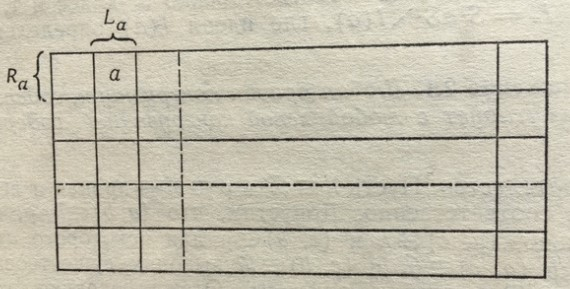
\includegraphics[width=0.9\textwidth]{egg_box}
		\caption{egg-box-диаграмма}
		\label{fig:egg_box}
	\end{figure}

	\section{Результаты работы}
	
	\subsection{Алгоритмы построения идеалов полугруппы по таблице Кэли}
	
	$\textit{Вход:}$ Полугруппа $S$ с таблицей Кэли размерности $N \times N$.

	$\textit{Выход:}$  Множество левых идеалов $L$, множество правых идеалов $R$ и множество двусторонних идеалов $DV$.

	\begin{enumerate} 
		\item Строится множество $elem\_for\_id$, которое содержит все комбинации из элементов полугруппы $S$, кроме повторяющихся комбинаций(элементы одинаковые, но идут в другом порядке) и тех, где встречаются одинаковые элементы.

		\item Все подмножества из $elem\_for\_id$ проверяются на условие правого идеала: если в непустом подмножестве $I \subset  S$ для любых $x \in I$,$y \in S$ выполняется условие: $xy \in I$, то данное подмножество является правым идеалом и добавляется в $R$.
		
		\item Все подмножества из $elem\_for\_id$ проверяются на условие левого идеала: если в непустом подмножестве $I \subset  S$ для любых $x \in I$,$y \in S$ выполняется условие: $yx \in I$, то данное подмножество является левым идеалом и добавляется в $L$.
		
		\item Если какое-то подмножество $I$ состоит и в $R$ и в $L$, то данное подмножество добавляется в $DV$.
		\item Возвращается множество левых идеалов $L$, множество правых идеалов $R$ и множество двусторонних идеалов $DV$.
	\end{enumerate} 
	
	Временная сложность алгоритма построения идеалов полугруппы по таблице Кэли = $O(2^n * n^3)$, где $n$ - количество элементов в полугруппе, ($2^n - 1$) - количество комбинаций в $elem\_for\_id$.
	
	\subsection{Алгоритм вычисления отношений Грина и построения «egg-box»-картины конечной полугруппы}
	
	$\textit{Вход:}$ Полугруппа $S$ с таблицей Кэли размерности $N \times N$.
	
	$\textit{Выход:}$  Отношения Грина $\Ra$, $\La$, $\Ja$, $\Ha$, $\Da$ и «egg-box»-картины.
	
	\begin{enumerate} 
		\item Для всех элементов $x,y \in S$ вычисляются правые идеалы $(x]$ и $(y]$, и, если они равны, пара $(x,y)$ добавляется в $\Ra$.
		
		\item Для всех элементов $x,y \in S$ вычисляются левые идеалы $[x)$ и $[y)$, и, если они равны, пара $(x,y)$ добавляется в $\La$.

		\item Для всех элементов $x,y \in S$ вычисляются левые идеалы $[x]$ и $[y]$, и, если они равны, пара $(x,y)$ добавляется в $\Ja$].

		\item Находится множество $\Ha$ с помощью пересечения множеств $\Ra$ и $\La$: $\Ha = \Ra \cap \La$.
			
		\item  Находится множество $\Da$ с помощью операции композиции: $\Da = \Ra \cdot \La$
		
		\item Вычисляются классы эквивалентности $\Da$, $\Ra$ и $\La$.
		
		\item Запускается цикл $for$ с $im$ от 0 до размера множества $\Da$. 
		
		\begin{enumerate}
			\item Проверяются все классы эквивалентности $\Ra$, и, если они совпали с $im$-тым элементом множества $\Da$, добавляются  в список списков vert.
			\item Проверяются все классы эквивалентности $\La$, и, если они совпали с $im$-тым элементом множества $\Da$, добавляются  в список списков hor.
			\item По vert и hor строится «egg-box»-картина следующим образом: На пересечении каждого подмножества из hor и каждого подмножества из vert стоят элементы, полученные пересечением этих двух подмножеств.
		\end{enumerate}
		
		\item Возвращаются отношения Грина $\Ra$, $\La$, $\Ja$, $\Ha$, $\Da$ и построенные «egg-box»-картины.
	\end{enumerate}

	Временная сложность алгоритма вычисления отношений Грина и построения «egg-box»-картины конечной полугруппы = $O(n^4)$, где $n$ - количество элементов в полугруппе.
	
	\section{Код программы}		
	
	 \begin{verbatim}
	 	
#include <iostream>
#include <vector>
#include <math.h>
#include <algorithm>
#include <string>
#include <iomanip>

using namespace std;

vector <vector<char>> all_elems;
int x = 0;

int CharInt(int N, char c, vector <char> mnojestvo) {
	for (int i = 0; i < N; i++)
	{
		if (mnojestvo[i] == c)
		return i;
	}
}

bool proverka_Ass(int N, char** keli, vector <char> mnojestvo) {
	bool prov = true;
	for (int x = 0; x < N; x++)
	{
		for (int y = 0; y < N; y++)
		{
			for (int z = 0; z < N; z++)
			{
				if (keli[x][CharInt(N, keli[y][z], mnojestvo)] 
				!= keli[CharInt(N, keli[x][y], mnojestvo)][z])
				prov = false;
			}
		}
	}
	return prov;
}

bool unique_elem(vector <char> ch, char elem) {
	for (int j = 0; j < ch.size(); j++) {
		if (elem == ch[j])
		return false;
	}
	return true;
}

bool unique_ideal(vector <char> ch, vector <vector <char>> all_ch) {
	for (int j = 0; j < all_ch.size(); j++) {
		if (ch == all_ch[j])
		return false;
	}
	return true;
}

bool unique_pair(pair <char, char> pair_ch, 
vector <pair <char, char>> pairs_ch) {
	for (int j = 0; j < pairs_ch.size(); j++) {
		if (pair_ch == pairs_ch[j])
		return false;
	}
	return true;
}

bool true_ideal(vector <char> X_i, vector <char> X_i_next) {
	if (X_i.size() != X_i_next.size())
	return true;
	return false;
}

bool vec2_in_vec1(vector <int> vec1, vector <int> vec2) {
	int elems_c = 0;
	for (int i = 0; i < vec2.size(); i++)
	{
		for (int i2 = 0; i2 < vec1.size(); i2++)
		{
			if (vec2[i] == vec1[i2])
			elems_c++;
		}
	}
	
	if (elems_c == vec2.size())
	{
		return true;
	}
	return false;
}

bool unique_symbols(vector <char> ch) {
	for (int j = 0; j < ch.size(); j++) {
		for (int j2 = 0; j2 < ch.size(); j2++) {
			if (j != j2 && ch[j] == ch[j2])
			return false;
		}
	}
	return true;
}

int this_el(char ch, vector<char> mnojestvo) {
	for (int i = 0; i < mnojestvo.size(); i++)
	if (ch == mnojestvo[i])
	return i;
}

bool not_uniq(char ch, vector<char> mnojestvo) {
	for (int i = 0; i < mnojestvo.size(); i++)
	if (ch == mnojestvo[i])
	return true;
}

bool is_ideal(vector <char> a, vector <char> mnojestvo, 
char** keli, bool s) {
	for (int i = 0; i < a.size(); i++)
	for (int j = 0; j < mnojestvo.size(); j++) {
		if (s == true) {
			if (!not_uniq(keli[this_el(a[i], mnojestvo)][j], a))
			return false;
		}
		else {
			if (!not_uniq(keli[j][this_el(a[i], mnojestvo)], a))
			return false;
		}
	}
	return true;
}

void ideal_f(int N, vector <char> mnojestvo, char** keli, 
vector <vector<char>> elems_for_id) {
	//ПРАВЫЕ ИДЕАЛЫ
	vector <vector <char>> res_pr;
	for (vector <char> a : elems_for_id)
	if (is_ideal(a, mnojestvo, keli, true))
	res_pr.push_back(a);
	cout << "Правые идеалы: ";
	for (int j = 0; j < res_pr.size(); j++) {
		vector <char> n_el = res_pr[j];
		if (!n_el.empty()) {
			cout << "{ ";
				for (int j = 0; j < n_el.size(); j++)
				if (j == n_el.size() - 1)
				cout << n_el[j];
				else
				cout << n_el[j] << " ";
				cout << " } ";
		}
	}
	cout << endl;
	
	//ЛЕВЫЕ ИДЕАЛЫ
	vector <vector <char>> res_lev;
	for (vector <char> a : elems_for_id)
	if (is_ideal(a, mnojestvo, keli, false))
	res_lev.push_back(a);
	cout << "Левые идеалы: ";
	for (int j = 0; j < res_lev.size(); j++) {
		vector <char> n_el = res_lev[j];
		if (!n_el.empty()) {
			cout << "{ ";
				for (int j = 0; j < n_el.size(); j++)
				if (j == n_el.size() - 1)
				cout << n_el[j];
				else
				cout << n_el[j] << " ";
				cout << " } ";
		}
	}
	cout << endl;
	
	//ДВУСТОРОННИЕ ИДЕАЛЫ
	vector <vector <char>> res_dvust;
	for (int i = 0; i < res_pr.size(); i++)
	{
		for (int i2 = 0; i2 < res_lev.size(); i2++)
		{
			if (res_pr[i] == res_lev[i2]) {
				res_dvust.push_back(res_pr[i]);
			}
		}
	}
	cout << "Двусторонние идеалы: ";
	for (int j = 0; j < res_dvust.size(); j++) {
		vector <char> n_el = res_dvust[j];
		if (!n_el.empty()) {
			cout << "{ ";
				for (int j = 0; j < n_el.size(); j++)
				if (j == n_el.size() - 1)
				cout << n_el[j];
				else
				cout << n_el[j] << " ";
				cout << " } ";
		}
	}
	cout << endl;
	return;
}

vector<vector <int> > fm;
void    fm_result(int N, vector <char> mnojestvo, int** matr)
{
	for (int i = 0; i < N; i++) {
		vector <int> vec;
		fm.push_back(vec);
		for (int j = 0; j < N; j++) {
			if (matr[i][j] == 1)
			{
				fm[fm.size() - 1].push_back(j + 1);
			}
		}
	}
	sort(fm.begin(), fm.end());
	fm.resize(unique(fm.begin(), fm.end()) - fm.begin());
	cout << "{ ";
		for (int i = 0; i < fm.size(); i++) {
			cout << "{";
				for (int j = 0; j < fm[i].size(); j++)
				{
					cout << mnojestvo[fm[i][j] - 1];
					if (j != fm[i].size() - 1)
					cout << ", ";
				}
				if (i == fm.size() - 1)
				cout << "} ";
			else
			cout << "}, ";
	}
	cout << "}" << endl;
}

bool find_in_vec_bool(int elem, vector <int> ch) {
for (int j = 0; j < ch.size(); j++) {
	if (elem == ch[j])
	return true;
}
return false;
}

bool vecs_2_bool(vector <int> ch1, vector <int> ch2) {
for (int j = 0; j < ch1.size(); j++) {
	for (int j2 = 0; j2 < ch2.size(); j2++) {
		if (ch1[j] == ch2[j2])
		return true;
	}
}
return false;
}

int vecs_2_elem(vector <int> ch1, vector <int> ch2) {
for (int j = 0; j < ch1.size(); j++) {
	for (int j2 = 0; j2 < ch2.size(); j2++) {
		if (ch1[j] == ch2[j2])
		return ch1[j];
	}
}
}

int find_in_vec(int elem, vector <int> ch) {
for (int j = 0; j < ch.size(); j++) {
	if (elem == ch[j])
	return elem;
}
}

void grina(int N, vector <char> mnojestvo, char** keli) {
// R
vector <pair <char, char>> R_pairs;
for (int j = 0; j < mnojestvo.size(); j++) {
	for (int j2 = 0; j2 < mnojestvo.size(); j2++) {
		vector <char> pr_1;
		pr_1.push_back(mnojestvo[j]);
		for (int k = 0; k < mnojestvo.size(); k++) {
			if (unique_elem(pr_1, keli[j][k]))
			pr_1.push_back(keli[j][k]);
		}
		vector <char> pr_2;
		pr_2.push_back(mnojestvo[j2]);
		for (int k = 0; k < mnojestvo.size(); k++) {
			if (unique_elem(pr_2, keli[j2][k]))
			pr_2.push_back(keli[j2][k]);
		}
		sort(pr_1.begin(), pr_1.end());
		sort(pr_2.begin(), pr_2.end());
		if (pr_1 == pr_2) {
			if (unique_pair(make_pair(mnojestvo[j], mnojestvo[j2]), R_pairs))
			R_pairs.push_back(make_pair(mnojestvo[j], mnojestvo[j2]));
		}
	}
}
// L
vector <pair <char, char>> L_pairs;
for (int j = 0; j < mnojestvo.size(); j++) {
	for (int j2 = 0; j2 < mnojestvo.size(); j2++) {
		vector <char> l_1;
		l_1.push_back(mnojestvo[j]);
		for (int k = 0; k < mnojestvo.size(); k++)
		if (unique_elem(l_1, keli[k][j]))
		l_1.push_back(keli[k][j]);
		vector <char> l_2;
		l_2.push_back(mnojestvo[j2]);
		for (int k = 0; k < mnojestvo.size(); k++)
		if (unique_elem(l_2, keli[k][j2]))
		l_2.push_back(keli[k][j2]);
		sort(l_1.begin(), l_1.end());
		sort(l_2.begin(), l_2.end());
		if (l_1 == l_2)
		if (unique_pair(make_pair(mnojestvo[j], mnojestvo[j2]), L_pairs))
		L_pairs.push_back(make_pair(mnojestvo[j], mnojestvo[j2]));
	}
}
// J

vector <pair <char, char>> J_pairs;
for (int j = 0; j < mnojestvo.size(); j++) {
	for (int j2 = 0; j2 < mnojestvo.size(); j2++) {
		vector <char> l_1;
		l_1.push_back(mnojestvo[j]);
		vector <char> l_1_s;
		for (int k = 0; k < mnojestvo.size(); k++)
		if (unique_elem(l_1_s, keli[k][j]))
		l_1_s.push_back(keli[k][j]);
		for (int i = 0; i < l_1_s.size(); i++) {
			for (int i2 = 0; i2 < mnojestvo.size(); i2++) {
				if (unique_elem(l_1, keli[this_el(l_1_s[i], mnojestvo)][i2]))
				l_1.push_back(keli[this_el(l_1_s[i], mnojestvo)][i2]);
			}
		}
		vector <char> l_2;
		l_2.push_back(mnojestvo[j2]);
		vector <char> l_2_s;
		for (int k = 0; k < mnojestvo.size(); k++)
		if (unique_elem(l_2_s, keli[k][j2]))
		l_2_s.push_back(keli[k][j2]);
		for (int i = 0; i < l_2_s.size(); i++) {
			for (int i2 = 0; i2 < mnojestvo.size(); i2++) {
				if (unique_elem(l_2, keli[this_el(l_2_s[i], mnojestvo)][i2]))
				l_2.push_back(keli[this_el(l_2_s[i], mnojestvo)][i2]);
			}
		}
		sort(l_1.begin(), l_1.end());
		sort(l_2.begin(), l_2.end());
		if (l_1 == l_2)
		if (unique_pair(make_pair(mnojestvo[j], mnojestvo[j2]), J_pairs))
		J_pairs.push_back(make_pair(mnojestvo[j], mnojestvo[j2]));
	}
}
// H
vector <pair <char, char>> H_pairs;
for (int i = 0; i < R_pairs.size(); i++)
{
	for (int i2 = 0; i2 < L_pairs.size(); i2++)
	{
		if (R_pairs[i] == L_pairs[i2])
		H_pairs.push_back(make_pair(R_pairs[i].first, R_pairs[i].second));
	}
}

cout << endl << "R = ";
for (int i = 0; i < R_pairs.size(); i++)
{
	cout << "( " << R_pairs[i].first << "," << R_pairs[i].second << " )";
}

cout << endl << "L = ";
for (int i = 0; i < L_pairs.size(); i++)
{
	cout << "( " << L_pairs[i].first << "," << L_pairs[i].second << " )";
}
cout << endl << "J = ";
for (int i = 0; i < J_pairs.size(); i++)
{
	cout << "( " << J_pairs[i].first << "," << J_pairs[i].second << " )";
}
cout << endl << "D = ";
for (int i = 0; i < J_pairs.size(); i++)
{
	cout << "( " << J_pairs[i].first << "," << J_pairs[i].second << " )";
}
cout << endl << "H   = ";
for (int i = 0; i < H_pairs.size(); i++)
{
	cout << "( " << H_pairs[i].first << "," << H_pairs[i].second << " )";
}
//бин матрицу для R строим
int** R_matr;
R_matr = new int* [N];
for (int i = 0; i < N; i++) {
	R_matr[i] = new int[N];
	for (int j = 0; j < N; j++) {
		R_matr[i][j] = 0;
	}
}
for (int i = 0; i < R_pairs.size(); i++)
{
	R_matr[this_el(R_pairs[i].first, mnojestvo)]
	[this_el(R_pairs[i].second, mnojestvo)] = 1;
}
cout << endl << "Матрица R: " << endl;
for (int i = 0; i < N; i++)
{
	for (int i2 = 0; i2 < N; i2++)
	{
		cout << R_matr[i][i2] << " ";
	}
	cout << endl;
}

//бин матрицу для L строим
int** L_matr;
L_matr = new int* [N];
for (int i = 0; i < N; i++) {
	L_matr[i] = new int[N];
	for (int j = 0; j < N; j++) {
		L_matr[i][j] = 0;
	}
}
for (int i = 0; i < L_pairs.size(); i++)
{
	L_matr[this_el(L_pairs[i].first, mnojestvo)]
	[this_el(L_pairs[i].second, mnojestvo)] = 1;
}
cout << "Матрица L: " << endl;
for (int i = 0; i < N; i++)
{
	for (int i2 = 0; i2 < N; i2++)
	{
		cout << L_matr[i][i2] << " ";
	}
	cout << endl;
}

//бин матрицу для D строим
int** J_matr;
J_matr = new int* [N];
for (int i = 0; i < N; i++) {
	J_matr[i] = new int[N];
	for (int j = 0; j < N; j++) {
		J_matr[i][j] = 0;
	}
}
for (int i = 0; i < J_pairs.size(); i++)
{
	J_matr[this_el(J_pairs[i].first, mnojestvo)]
	[this_el(J_pairs[i].second, mnojestvo)] = 1;
}
cout << "Матрица D: " << endl;
for (int i = 0; i < N; i++)
{
	for (int i2 = 0; i2 < N; i2++)
	{
		cout << J_matr[i][i2] << " ";
	}
	cout << endl;
}

//классы эквивалентности
cout << "Классы эквивалентности R:  ";
fm_result(N, mnojestvo, R_matr);
vector<vector <int> > R_fm = fm;
fm.clear();
cout << "Классы эквивалентности L:  ";
fm_result(N, mnojestvo, L_matr);
vector<vector <int> > L_fm = fm;
fm.clear();
cout << "Классы эквивалентности D:  ";
fm_result(N, mnojestvo, J_matr);
vector<vector <int> > D_fm = fm;
fm.clear();

//Строим egg-box
for (int im = 0; im < D_fm.size(); im++) {
	vector <vector <int>> vert;
	vector <vector <int>> hor;
	for (int i = 0; i < R_fm.size(); i++)
	{
		if (vec2_in_vec1(D_fm[im], R_fm[i]))
		vert.push_back(R_fm[i]);
	}
	for (int i = 0; i < L_fm.size(); i++)
	{
		if (vec2_in_vec1(D_fm[im], L_fm[i]))
		hor.push_back(L_fm[i]);
	}
	vector <vector <char>> egg_box_1;
	for (int j = 0; j < vert.size(); j++) {
		vector <char> in_egg_box(hor.size(), '0');
		egg_box_1.push_back(in_egg_box);
	}
	for (int i = 0; i < vert.size(); i++)
	{
		for (int i3 = 0; i3 < hor.size(); i3++)
		{
			if (vecs_2_bool(vert[i], hor[i3])) {
				egg_box_1[i][i3] = mnojestvo[vecs_2_elem(vert[i], hor[i3]) - 1];
			}
		}
	}
	cout << "egg box: " << endl;
	cout << setw(vert[0].size() * 4);
	for (int i = 0; i < hor.size(); i++) {
		cout << "{";
			for (int j = 0; j < hor[i].size(); j++)
			{
				cout << mnojestvo[hor[i][j] - 1];
				if (j != hor[i].size() - 1)
				cout << ", ";
			}
			if (i == hor.size() - 1)
			cout << "} ";
		else
		cout << "} ";
}
cout << endl;
for (int i = 0; i < egg_box_1.size(); i++)
{
	cout << "{";
		for (int j = 0; j < vert[i].size(); j++)
		{
			cout << mnojestvo[vert[i][j] - 1];
			if (j != vert[i].size() - 1)
			cout << ", ";
		}
		cout << "}  ";
	for (int i2 = 0; i2 < egg_box_1[i].size(); i2++)
	{
		cout << setw(hor[i2].size() + 2) << egg_box_1[i][i2] << " ";
	}
	cout << endl;
}
}
}

void proverka_1(int N, vector <char> mnojestvo, char** keli, 
vector <vector<char>> elems_for_id) {

cout << endl;
if (proverka_Ass(N, keli, mnojestvo) == true) {
ideal_f(N, mnojestvo, keli, elems_for_id);
}
else
cout << "Не ассоциативна" << endl;

}

void proverka_2(int N, vector <char> mnojestvo, char** keli) {

cout << endl;
if (proverka_Ass(N, keli, mnojestvo) == true) {
grina(N, mnojestvo, keli);
}
else
cout << "Не ассоциативна" << endl;

}

void next_comb(long long num, size_t radix, vector<size_t>& idxs) {
for (int i = idxs.size(); i > 0; --i) {
idxs[i - 1] = num % radix;
num /= radix;
}
}

void gen2(const vector<char>& alf, size_t n) {
size_t alf_len = alf.size();
long long total = [](size_t bas, size_t exp) { long long pow = 1LL;
	  while (exp-- > 0) pow *= bas; return pow; }(alf_len, n);
vector<size_t> indexes(n);

for (long long i = 0; i < total; ++i) {
next_comb(i, alf_len, indexes);
for (size_t j = 0; j < n; ++j) {
	vector <char> dd(0);
	all_elems.push_back(dd);
	all_elems[x].push_back(alf[indexes[j]]);
}
x++;
}
}

int main()
{
setlocale(LC_ALL, "Rus");
vector <char> mnojestvo;
vector <char> podmnojestvo;
vector <string> A;
vector <string> A_ofr;
vector < vector < vector <int> > > all_matr;
vector < vector < vector <int> > > res_all_matr;
int sposob, i, j, N, M, T, matr_count, R_count, R;
int max_w = 0;
cout << "Введите, что хотите сделать: " << endl;
cout << "1 - построения идеалов полугруппы по таблице Кэли" << endl;
cout << "2 - алгоритм вычисления отношений Грина и 
построения «egg-box»-картины конечной полугруппы" << endl;
cin >> sposob;

if (sposob == 1)
{
vector <char> mnojestvo;
size_t s = 1;
int N;
cout << "Введите размерность полугруппы: " << endl;
cin >> N;
if (N == 0) {
	cout << "Ошибка";
	return 0;
}
cout << "Введите множество для полугруппы S: " << endl;
char vv;
for (int i = 0; i < N; i++) {
	cin >> vv;
	mnojestvo.push_back(vv);
}

while (s != N) {
	gen2(mnojestvo, s);
	s++;
}
vector <vector<char>> elems_for_id;
all_elems.push_back(mnojestvo);
for (int i = 0; i < all_elems.size(); i++)
{
	vector<char> elem_now = all_elems[i];
	sort(elem_now.begin(), elem_now.end());
	if (unique_ideal(elem_now, elems_for_id) && unique_symbols(elem_now)) {
		elems_for_id.push_back(elem_now);
	}
}
char** keli;
keli = new char* [N];
cout << "Таблица Кэли полугруппы S: " << endl;
for (int i = 0; i < N; i++) {
	keli[i] = new char[N];
	for (int j = 0; j < N; j++) {
		cin >> keli[i][j];
	}
}
proverka_1(N, mnojestvo, keli, elems_for_id);
}
else if (sposob == 2)
{

vector <char> mnojestvo;
int N;
cout << "Введите размерность полугруппы: " << endl;
cin >> N;
if (N == 0) {
	cout << "Ошибка";
	return 0;
}
cout << "Введите множество для полугруппы S: " << endl;
char vv;
for (int i = 0; i < N; i++) {
	cin >> vv;
	mnojestvo.push_back(vv);
}

char** keli;
keli = new char* [N];
cout << "Таблица Кэли полугруппы S: " << endl;
for (int i = 0; i < N; i++) {
	keli[i] = new char[N];
	for (int j = 0; j < N; j++) {
		cin >> keli[i][j];
	}
}
proverka_2(N, mnojestvo, keli);
}
else
cout << "Ошибка" << endl;

cout << endl;
}


	
	\end{verbatim}
	
	\section{Результаты тестирования программ}
	
	Тестирование №1:
	
Построение идеалов полугруппы по таблице Кэли.

	\begin{figure}[H]
		\centering
		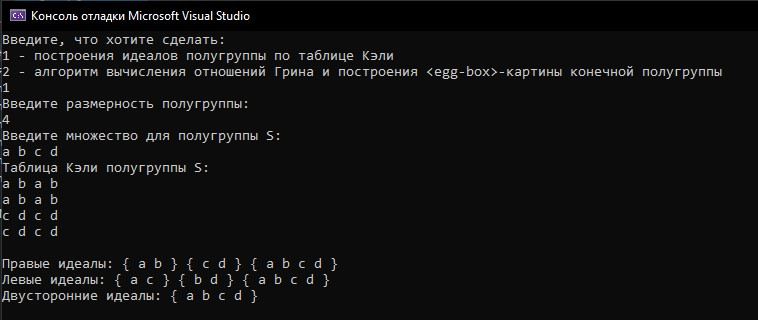
\includegraphics[width=0.9\textwidth]{test_1}
		\caption{Тестировние №1}
		\label{fig:test_1}
	\end{figure}
	
	Тестирование №2:
	
Вычисления отношений Грина и построение «egg-box»-картины конечной полугруппы.
	
	\begin{figure}[H]
		\centering
		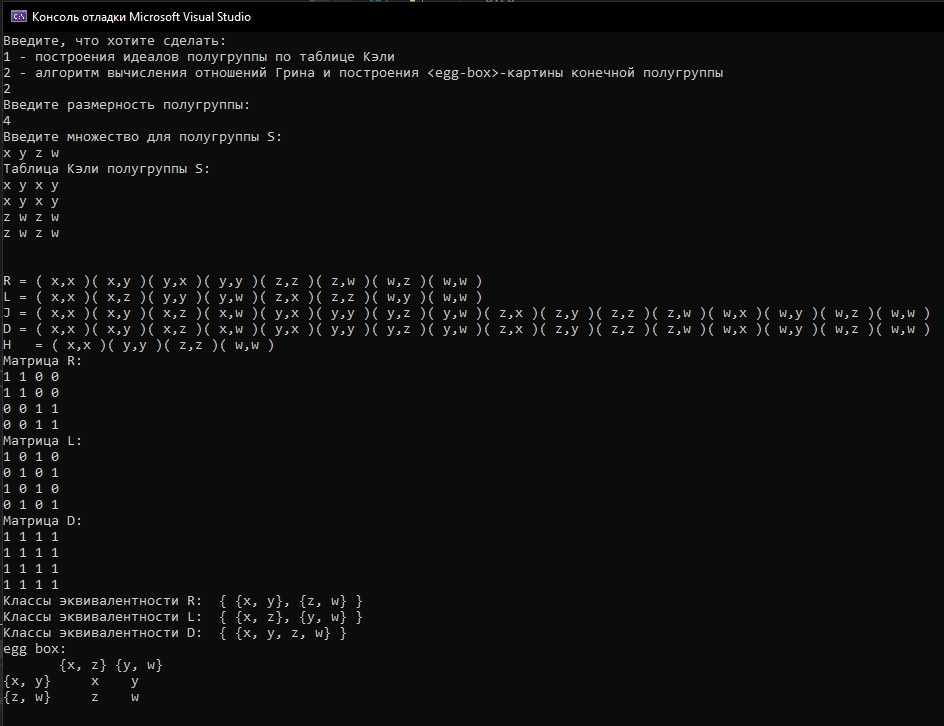
\includegraphics[width=0.9\textwidth]{test_2}
		\caption{Тестировние №2}
		\label{fig:test_2}
	\end{figure}

	\newpage
	\conclusion %заключение
	
	В данной лабораторной работе были рассмотрены и изучены следующие темы: понятия идеалов полугруппы, понятия и свойства отношений Грина на полугруппах. Во второй части работы были реализованы: алгоритмы построения идеалов полугруппы по таблице Кэли, алгоритмы вычисления отношений Грина и построения «egg-box»-картины конечной полугруппы.  
	  
	
	
	
\end{document}